% Options for packages loaded elsewhere
\PassOptionsToPackage{unicode}{hyperref}
\PassOptionsToPackage{hyphens}{url}
%
\documentclass[
]{article}
\usepackage{lmodern}
\usepackage{amssymb,amsmath}
\usepackage{ifxetex,ifluatex}
\ifnum 0\ifxetex 1\fi\ifluatex 1\fi=0 % if pdftex
  \usepackage[T1]{fontenc}
  \usepackage[utf8]{inputenc}
  \usepackage{textcomp} % provide euro and other symbols
\else % if luatex or xetex
  \usepackage{unicode-math}
  \defaultfontfeatures{Scale=MatchLowercase}
  \defaultfontfeatures[\rmfamily]{Ligatures=TeX,Scale=1}
\fi
% Use upquote if available, for straight quotes in verbatim environments
\IfFileExists{upquote.sty}{\usepackage{upquote}}{}
\IfFileExists{microtype.sty}{% use microtype if available
  \usepackage[]{microtype}
  \UseMicrotypeSet[protrusion]{basicmath} % disable protrusion for tt fonts
}{}
\makeatletter
\@ifundefined{KOMAClassName}{% if non-KOMA class
  \IfFileExists{parskip.sty}{%
    \usepackage{parskip}
  }{% else
    \setlength{\parindent}{0pt}
    \setlength{\parskip}{6pt plus 2pt minus 1pt}}
}{% if KOMA class
  \KOMAoptions{parskip=half}}
\makeatother
\usepackage{xcolor}
\IfFileExists{xurl.sty}{\usepackage{xurl}}{} % add URL line breaks if available
\IfFileExists{bookmark.sty}{\usepackage{bookmark}}{\usepackage{hyperref}}
\hypersetup{
  pdftitle={Surgical sutures},
  pdfauthor={Andrew J. Sims},
  hidelinks,
  pdfcreator={LaTeX via pandoc}}
\urlstyle{same} % disable monospaced font for URLs
\usepackage[margin=1in]{geometry}
\usepackage{longtable,booktabs}
% Correct order of tables after \paragraph or \subparagraph
\usepackage{etoolbox}
\makeatletter
\patchcmd\longtable{\par}{\if@noskipsec\mbox{}\fi\par}{}{}
\makeatother
% Allow footnotes in longtable head/foot
\IfFileExists{footnotehyper.sty}{\usepackage{footnotehyper}}{\usepackage{footnote}}
\makesavenoteenv{longtable}
\usepackage{graphicx,grffile}
\makeatletter
\def\maxwidth{\ifdim\Gin@nat@width>\linewidth\linewidth\else\Gin@nat@width\fi}
\def\maxheight{\ifdim\Gin@nat@height>\textheight\textheight\else\Gin@nat@height\fi}
\makeatother
% Scale images if necessary, so that they will not overflow the page
% margins by default, and it is still possible to overwrite the defaults
% using explicit options in \includegraphics[width, height, ...]{}
\setkeys{Gin}{width=\maxwidth,height=\maxheight,keepaspectratio}
% Set default figure placement to htbp
\makeatletter
\def\fps@figure{htbp}
\makeatother
\setlength{\emergencystretch}{3em} % prevent overfull lines
\providecommand{\tightlist}{%
  \setlength{\itemsep}{0pt}\setlength{\parskip}{0pt}}
\setcounter{secnumdepth}{-\maxdimen} % remove section numbering

\title{Surgical sutures}
\author{Andrew J. Sims}
\date{February 2021}

\begin{document}
\maketitle

\hypertarget{introduction}{%
\section{Introduction}\label{introduction}}

Leaper \emph{et al} {[}1{]} presented a model that compared
antimicrobial surgical sutures (absorbable sutures impregnated with
triclosan, TCS) with standard care, absorbable sutures with no
antimicrobial impregnation (NCS). The model was evaluated in three
scenarios:

\begin{itemize}
\tightlist
\item
  clean wounds;
\item
  clean-contaminated wounds;
\item
  contaminated and dirty wounds
\end{itemize}

\hypertarget{scenario-1-clean-wounds}{%
\section{Scenario 1: clean wounds}\label{scenario-1-clean-wounds}}

\hypertarget{model-structure}{%
\subsection{Model structure}\label{model-structure}}

The decision tree defined by Leaper \emph{et al} {[}1{]} is shown in
figure 1.

\begin{figure}

{\centering 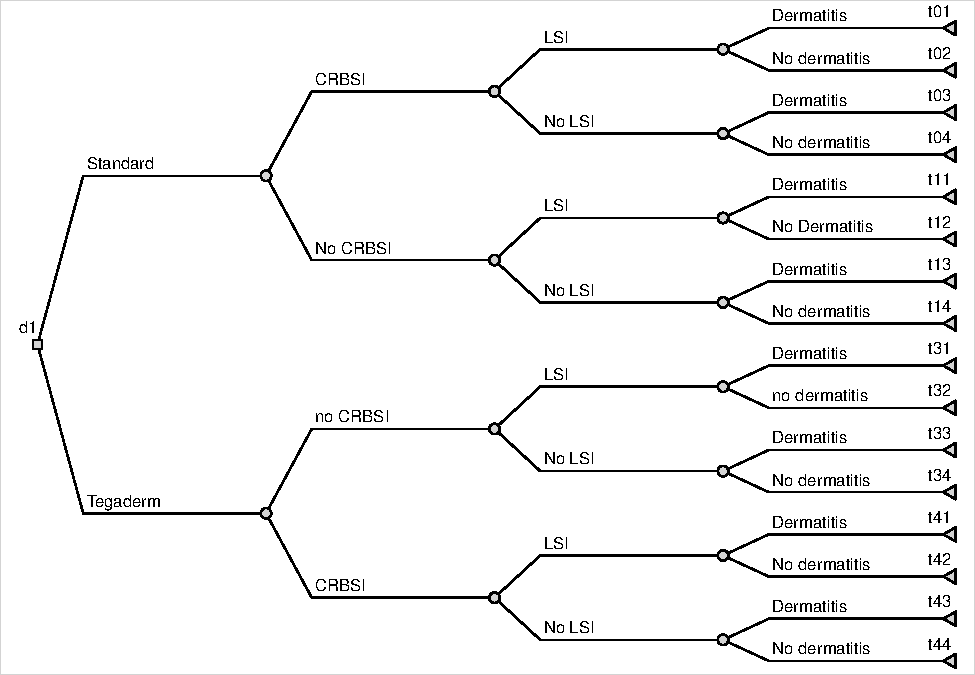
\includegraphics{Sutures_files/figure-latex/draw-1} 

}

\caption{Decision tree for all scenarios.}\label{fig:draw}
\end{figure}

\hypertarget{model-variables}{%
\subsection{Model variables}\label{model-variables}}

The model had six input variables (Table 1): the probability of an SSI
with NCS, the risk ratio of an SSI with TCS compared with NCS, cost of
TCS, cost of NCS, number of sutures per surgical procedure and cost of
an admission with diagnosis of infection.

\begin{longtable}[]{@{}lllrrr@{}}
\caption{Model inputs}\tabularnewline
\toprule
\begin{minipage}[b]{0.16\columnwidth}\raggedright
Description\strut
\end{minipage} & \begin{minipage}[b]{0.09\columnwidth}\raggedright
Units\strut
\end{minipage} & \begin{minipage}[b]{0.19\columnwidth}\raggedright
Distribution\strut
\end{minipage} & \begin{minipage}[b]{0.08\columnwidth}\raggedleft
Mean\strut
\end{minipage} & \begin{minipage}[b]{0.09\columnwidth}\raggedleft
Q2.5\strut
\end{minipage} & \begin{minipage}[b]{0.09\columnwidth}\raggedleft
Q97.5\strut
\end{minipage}\tabularnewline
\midrule
\endfirsthead
\toprule
\begin{minipage}[b]{0.16\columnwidth}\raggedright
Description\strut
\end{minipage} & \begin{minipage}[b]{0.09\columnwidth}\raggedright
Units\strut
\end{minipage} & \begin{minipage}[b]{0.19\columnwidth}\raggedright
Distribution\strut
\end{minipage} & \begin{minipage}[b]{0.08\columnwidth}\raggedleft
Mean\strut
\end{minipage} & \begin{minipage}[b]{0.09\columnwidth}\raggedleft
Q2.5\strut
\end{minipage} & \begin{minipage}[b]{0.09\columnwidth}\raggedleft
Q97.5\strut
\end{minipage}\tabularnewline
\midrule
\endhead
\begin{minipage}[t]{0.16\columnwidth}\raggedright
VICRYL plus\strut
\end{minipage} & \begin{minipage}[t]{0.09\columnwidth}\raggedright
GBP\strut
\end{minipage} & \begin{minipage}[t]{0.19\columnwidth}\raggedright
Ga(100,0.036)\strut
\end{minipage} & \begin{minipage}[t]{0.08\columnwidth}\raggedleft
3.63\strut
\end{minipage} & \begin{minipage}[t]{0.09\columnwidth}\raggedleft
2.954\strut
\end{minipage} & \begin{minipage}[t]{0.09\columnwidth}\raggedleft
4.375\strut
\end{minipage}\tabularnewline
\begin{minipage}[t]{0.16\columnwidth}\raggedright
VICRYL\strut
\end{minipage} & \begin{minipage}[t]{0.09\columnwidth}\raggedright
GBP\strut
\end{minipage} & \begin{minipage}[t]{0.19\columnwidth}\raggedright
Ga(100,0.029)\strut
\end{minipage} & \begin{minipage}[t]{0.08\columnwidth}\raggedleft
2.88\strut
\end{minipage} & \begin{minipage}[t]{0.09\columnwidth}\raggedleft
2.343\strut
\end{minipage} & \begin{minipage}[t]{0.09\columnwidth}\raggedleft
3.471\strut
\end{minipage}\tabularnewline
\bottomrule
\end{longtable}

\hypertarget{results}{%
\section{Results}\label{results}}

\begin{longtable}[]{@{}cccccc@{}}
\toprule
\begin{minipage}[b]{0.07\columnwidth}\centering
Run\strut
\end{minipage} & \begin{minipage}[b]{0.23\columnwidth}\centering
Suture\strut
\end{minipage} & \begin{minipage}[b]{0.16\columnwidth}\centering
Probability\strut
\end{minipage} & \begin{minipage}[b]{0.09\columnwidth}\centering
Cost\strut
\end{minipage} & \begin{minipage}[b]{0.12\columnwidth}\centering
Benefit\strut
\end{minipage} & \begin{minipage}[b]{0.12\columnwidth}\centering
Utility\strut
\end{minipage}\tabularnewline
\midrule
\endhead
\begin{minipage}[t]{0.07\columnwidth}\centering
1\strut
\end{minipage} & \begin{minipage}[t]{0.23\columnwidth}\centering
Antimicrobial\strut
\end{minipage} & \begin{minipage}[t]{0.16\columnwidth}\centering
1\strut
\end{minipage} & \begin{minipage}[t]{0.09\columnwidth}\centering
208.3\strut
\end{minipage} & \begin{minipage}[t]{0.12\columnwidth}\centering
0\strut
\end{minipage} & \begin{minipage}[t]{0.12\columnwidth}\centering
1\strut
\end{minipage}\tabularnewline
\begin{minipage}[t]{0.07\columnwidth}\centering
1\strut
\end{minipage} & \begin{minipage}[t]{0.23\columnwidth}\centering
Non-antimicrobial\strut
\end{minipage} & \begin{minipage}[t]{0.16\columnwidth}\centering
1\strut
\end{minipage} & \begin{minipage}[t]{0.09\columnwidth}\centering
305.8\strut
\end{minipage} & \begin{minipage}[t]{0.12\columnwidth}\centering
0\strut
\end{minipage} & \begin{minipage}[t]{0.12\columnwidth}\centering
1\strut
\end{minipage}\tabularnewline
\bottomrule
\end{longtable}

\hypertarget{references}{%
\section*{References}\label{references}}
\addcontentsline{toc}{section}{References}

\hypertarget{refs}{}
\leavevmode\hypertarget{ref-leaper2017}{}%
1 Leaper DJ, Edmiston Jr CE, Holy CE. Meta-analysis of the potential
economic impact following introduction of absorbable antimicrobial
sutures. \emph{BJS (British Journal of Surgery)}
2017;\textbf{104}:e134--44.
doi:\href{https://doi.org/10.1002/bjs.10443}{10.1002/bjs.10443}

\end{document}
